\documentclass[12pt,letterpaper,noanswers]{exam}
\usepackage[usenames,dvipsnames,svgnames,table]{xcolor}
\usepackage[margin=0.9in]{geometry}
\renewcommand{\familydefault}{\sfdefault}
\usepackage{multicol}
\pagestyle{head}
\header{AM 108 Class 30}{}{Universality}
\runningheadrule
\headrule
\usepackage{graphicx} % more modern
\usepackage{amsmath} 
\usepackage{amssymb} 
\usepackage{hyperref}
\usepackage{tcolorbox}

\begin{document}
 \pdfpageheight 11in 
  \pdfpagewidth 8.5in

\noindent 




\begin{itemize}
\itemsep0em
\item You have a project weekly log due Friday (and again next Friday).  Your project work is replacing the problem set.
\item There is a new skill check for Friday.
\item The Quiz 02 Follow Up is due Mon Nov 23rd.  The retake, if assigned to you, is due Thurs Dec 3rd.  Request a different due date via private message on Piazza, if needed.
\end{itemize}

\hrule
\vspace{0.2cm}



\noindent\textbf{Teams}



\noindent \textbf{Teams 3 and 4}: Post screenshots of your work to the course Google Drive today.  Include words, labels, and other short notes that might make those solutions useful to you or your classmates.  Find the link in Canvas (or here: \url{https://drive.google.com/drive/u/0/folders/1GcpwvKHD4tMecpFQ4lNxN_r5Ylj7YHbd})


\vspace{0.2cm}

\hrule
\vspace{0.2cm}


\noindent\textbf{Big picture}

The parameter spacing ratio, $\delta$ (and the size of the splittings, $\alpha$), occurs in the orbit diagrams of many (unimodal) maps.  Why does this spacing occur so universally?  

\vspace{0.2cm}
\hrule
\vspace{0.2cm}

\noindent \textbf{Extra vocabulary / extra facts:}
\begin{tcolorbox}
You may have studied the \textbf{central limit theorem} in another class.  The central limit theorem roughly says that when you add independent random variables that obey a distribution function, $f$, the (normalized) sum tends towards a Gaussian distribution, $g$.

The Gaussian distribution is an example of a \textbf{universal function}.  The same $g$ arises for many different distribution functions $f$. 
\end{tcolorbox}


\vspace{0.2cm}
\hrule
\vspace{0.2cm}

\noindent\textbf{Your questions}
\begin{enumerate}
    \item Do $\alpha$ and $\delta$ have meaning in other contexts?  What is important about these universal scaling constants for studying chaos?
    \item What is the value of finding a universal limiting function?
    \item The order of the maximum of $f$ is never forgotten in the renormalization process. How does that impact the universality of this?
    \item For Lorenz and Rossler, we can connect the systems to a map that we can then study.  How would the analysis of chaos change when there isn't a map / the chaotic attractor is not a fractal?
\end{enumerate}


\vspace{0.2cm}
\hrule
\vspace{0.2cm}

\noindent\textbf{Skill Check C31 practice}
\begin{questions}
\item Skill check C28 retake.

\item Consider the map $x_{n+1} = r\sin x_n$ with $0\leq x \leq \pi$.  Find $x^*$ and $r_0$ such that $x^*$ is a superstable fixed point of the map at $r = r_0$.
\end{questions}

\vspace{0.2cm}

\hrule
\vspace{0.2cm}

\noindent\textbf{Skill Check C31 Practice Solution}

At a superstable fixed point, $f'(x) = 0$.  $f(x) = r\sin x$ and $f'(x) = r\cos x$.  For $x \in [0,\pi]$, $\cos x = 0$ when $x = \pi/2$.  We want $x^* = \pi/2$ to be a fixed point of the map (in order to have a superstable fixed point).  We have $\pi/2 = r_0\sin\pi/2 = r$, so $r_0 = \pi/2$.  


\vspace{0.2cm}

\hrule
\vspace{0.2cm}


\noindent\textbf{Questions}

\noindent \ \ 0.  Share a movie you found interesting with your team, and write your names on the slide.

\begin{questions}
\question The shifted logistic map is shown for four values of $r$.  

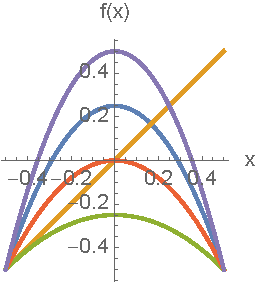
\includegraphics{img/191113-C29p1.pdf}

\begin{parts}
\item A superstable fixed point exists when $f'(x^*) = 0$.  Show that for this shifted logistic map the superstable fixed point will occur when $x = 0$ is a fixed point of the map.

\item Why is there only one value of $r$ for which there is a superstable fixed point?
\end{parts}

\question 

\begin{parts}

\item Show that for the shifted logistic map, a superstable period-$k$ orbit will occur when $x = 0$ is one of the points in the orbit.

\part Shown below are $f(x)$, $f(f(x))$, and $f^4(x)$ for three different values of $r$.  

In the $f(x)$ plot, $x = 0$ is a superstable period-1 point for $r = r_0$.  
\begin{itemize}
    \item Given that $r_1 \neq r_0$, argue that $x = 0$ is part of a superstable period-2 orbit when $r = r_1$.
    \item Given that $r_2 \neq r_1$ and $r_2\neq r_0$, argue that $x = 0$ is part of a superstable period-4 orbit when $r = r_2$.
\end{itemize}



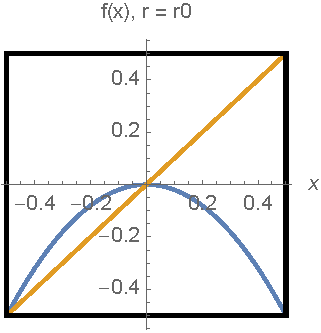
\includegraphics[width=0.23\textwidth]{img/191113-C29p2A.pdf}
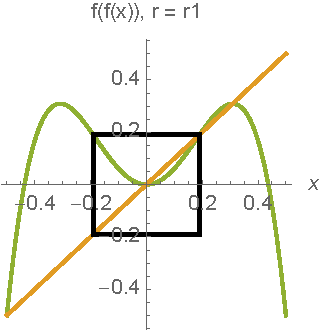
\includegraphics[width=0.23\textwidth]{img/191113-C29p2b.pdf}
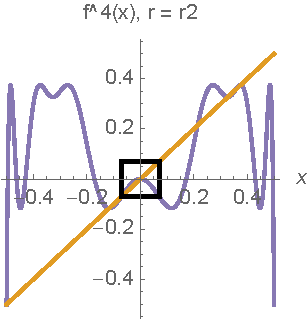
\includegraphics[width=0.23\textwidth]{img/191113-C29p3a.pdf}

\part

At the superstable value of $r$, $f(f(x))$ has a very similar shape to $f(x)$ close to $x = 0$.  Rescaling to zoom in:

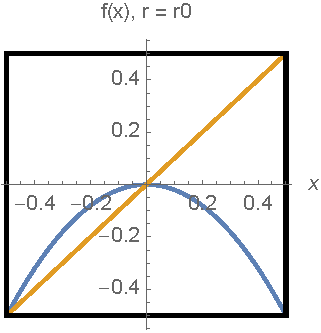
\includegraphics[width=0.21\textwidth]{img/191113-C29p2A.pdf}
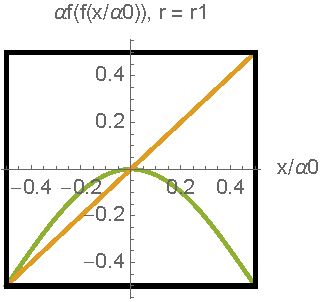
\includegraphics[width=0.23\textwidth]{img/191113-C29p2c.pdf}

Given this, why would you expect $f(f(x))$ at $r = r_1$ to experience a similar sequence of period doublings to $f(x)$ at $r = r_0$?

\item 
At the superstable value of $r$, $f^4(x)$ has a very similar shape to $f(x)$ close to $x = 0$.  Rescaling to zoom in:

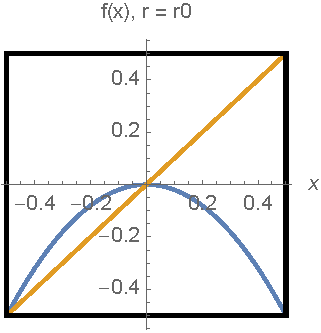
\includegraphics[width=0.21\textwidth]{img/191113-C29p2A.pdf}
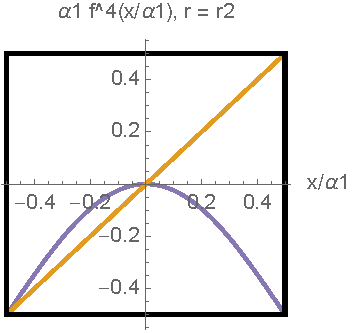
\includegraphics[width=0.23\textwidth]{img/191113-C29p3b.pdf}

Each period doubling and rescaling gets us closer to a universal shape to the hump in the map!

The functions are approaching a universal function, called $g_0$.

% 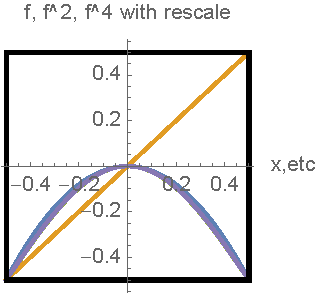
\includegraphics{img/191113-C29p3c.pdf}

$g_0(x) = \lim_{n\rightarrow\infty} \alpha^nf^{2^n}\left(x/\alpha^n,r_n\right)$ where $\alpha$ is the rescaling factor.

The function $g_0(x)$ is a \textbf{universal function}.  It will arise for many different starting functions $f$.

How might approaching the same universal function $g_0$ for two different starting maps contribute to the period-doubling sequence looking similar for two different orbit diagrams?


\end{parts}

\question We can create a sequence of $r$ values $r_0, r_1, r_2, r_3, ..., r_k, ...$ that are associated with superstable orbits of period $2^k$.

\begin{parts}
\item Above, we considered $f(x; r_0)$, $f^2(x; r_1)$; $f^4(x; r_2)$, and rescalings of these $\alpha^k f^{2^k}(x/\alpha^k; r_k)$.  These rescaled functions looked very similar to each other and approached a limiting function, $g_0$.

Now consider $f(x; r_1)$, $f^2(x; r_2)$; $f^4(x; r_3)$, and rescalings of these, $\alpha^k f^{2^k}(x/\alpha^k; r_{k+})$.

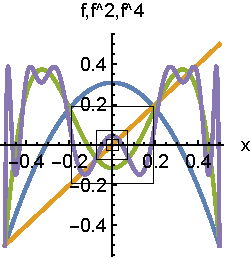
\includegraphics{img/20191113-C29p7a.pdf}
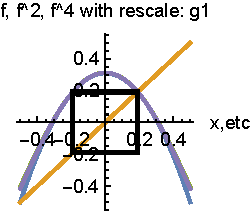
\includegraphics{img/20191113-C29p7b.pdf}

How do these iterates looks when rescaled?  Why isn't there a superstable fixed point showing up?

We have a second universal function, $g_1(x) = \lim_{n\rightarrow\infty} \alpha^nf^{2^n}\left(x/\alpha^n,r_{n+1}\right)$

\part Now consider $f(x; r_6)$, $f^2(x; r_7)$, $f^4(x; r_8)$.  The maps are shown on the left and the rescalings are shown on the right.  How do these iterates looks when rescaled?

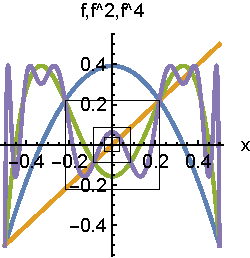
\includegraphics{img/20191113-C29p12a.pdf}
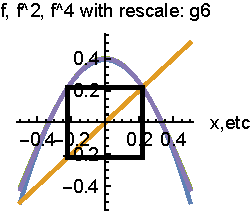
\includegraphics{img/20191113-C29p12b.pdf}

We can write $g_6(x) = \lim_{n\rightarrow\infty} \alpha^nf^{2^n}\left(x/\alpha^n,r_{n+6}\right)$ (another universal function!)

\part We have a family of universal functions, $g_k$.

Consider $f(x; r_\infty)$, $f^2(x; r_\infty)$, $f^4(x; r_\infty)$, where $r_\infty = \lim_{k\rightarrow\infty} r_k$.  The rescalings are shown again on the right.

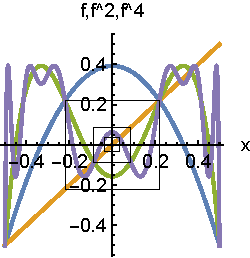
\includegraphics{img/20191113-C29p13a.pdf}
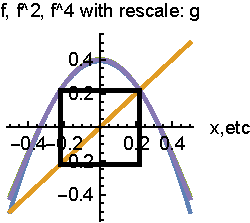
\includegraphics{img/20191113-C29p13b.pdf}

We can write $g(x) =  \alpha g^2(x/\alpha)$.  This one is simpler to write down: it is specified by a \textbf{functional equation.}
By shifting $f(x)$ we can set the maximum of the quadratic hump to be at $x = 0$, so require $g'(0) = 0$.

Near the origin, $g(x)$ looks parabolic.  Think of how wiggly $f^4(x)$ was.  Away from the origin $g(x)$ is also very wiggly.  Show that if $x^*$ is a fixed point of $g(x)$ then so is $\alpha x^*$.  Argue that this means that $g(x)$ crosses the line $y=x$ infinitely many times.

\end{parts}

\question A closed form for the universal function $g(x)$ is not known.   You can approximate the solution to the functional equation using a power series.  We have an even function, so $g(x) = 1+c_2x^2+c_4x^4+...$.  Suppose $g(x) \approx 1+c_2x^2$.  Find an expression for $c_2$ and for $\alpha$.  \emph{Neglect terms with $x^4$ or higher}.

\question (Further exploration of $g(x)$) 

Here's some code for building out the $g(x)$ function.  It only gets you to $g(x)$ for $-3<x<3$, though, before Mathematica stops really converging on the calculations in a reasonable amount of time.  (To check how well it is doing, I plot $g(x)$ and $\alpha g(g(x/\alpha))$ on the same axes and see the extent to which they match).

\begin{verbatim}
num = 1;
acestimate = {a -> -2.53, c[1] -> -1.52};
Do[b[x_] = 
  1 + Total[Flatten[Table[c[val] x^{2 val}, {val, 1, num}]]];
 cf = CoefficientList[Expand[a b[b[x/a]] - b[x]], x];
 cftruncate = cf[[1 ;; 2*num + 1]];
 varlist = 
  Flatten[{{{a, a /. acestimate}}, 
    Table[{c[val], c[val] /. acestimate}, {val, 1, num}]}, 1];
 acestimate = FindRoot[cftruncate[[1 ;; -1 ;; 2]] == 0, varlist]; 
 AppendTo[acestimate, c[num + 1] -> 0.5], {num, 1, 7}
 ]
acestimate
\end{verbatim}


\end{questions}

\end{document}